\subsection{Luz entrando por la cara plana}
En esta primera serie la luz va del aire al acrílico. Los ángulos medidos están en la tabla \ref{tab:plana}, junto con sus senos y el índice que resulta de cada pareja, calculado como $n = \sin\theta_i / \sin\theta_t$.

\begin{center}
\begin{tabular}{ccccc}
\hline
$\theta_i$ & $\theta_t$ & $\sin\theta_i$ & $\sin\theta_t$ & $n$ \\
(grados) & (grados) & & & \\
\hline
0  & 0  & 0      & 0      & ---   \\
5  & 5  & 0.0872 & 0.0872 & 1.000 \\
10 & 8  & 0.1736 & 0.1392 & 1.248 \\
15 & 12 & 0.2588 & 0.2079 & 1.245 \\
20 & 16 & 0.3420 & 0.2756 & 1.241 \\
25 & 20 & 0.4226 & 0.3420 & 1.236 \\
30 & 23 & 0.5000 & 0.3907 & 1.280 \\
35 & 25 & 0.5736 & 0.4226 & 1.357 \\
40 & 28 & 0.6428 & 0.4695 & 1.369 \\
45 & 31 & 0.7071 & 0.5150 & 1.373 \\
50 & 34 & 0.7660 & 0.5592 & 1.370 \\
55 & 37 & 0.8192 & 0.6018 & 1.361 \\
60 & 40 & 0.8660 & 0.6428 & 1.347 \\
65 & 42 & 0.9063 & 0.6691 & 1.354 \\
70 & 44 & 0.9397 & 0.6947 & 1.353 \\
75 & 45 & 0.9659 & 0.7071 & 1.366 \\
80 & 46 & 0.9848 & 0.7193 & 1.369 \\
85 & 47 & 0.9962 & 0.7314 & 1.362 \\
89 & 48 & 0.9998 & 0.7431 & 1.345 \\
\hline
\end{tabular}
\captionof{table}{Ángulos de incidencia y de refracción con la luz entrando por la cara plana.}
\label{tab:plana}
\end{center}

El rayo siempre se acercó a la normal. Incluso con la luz llegando casi rasante, a 89 grados, el rayo dentro del acrílico no pasó de 48 grados.

Siguiendo la ecuación \eqref{eq:recta}, se graficó $\sin\theta_i$ contra $\sin\theta_t$ y se ajustó una recta que pasa por el origen, mostrada en la figura \ref{fig:plana}:
\begin{equation}
\sin\theta_i = 1.351 \, \sin\theta_t , \qquad R^2 = 0.9972 .
\label{eq:ajuste_plana}
\end{equation}

\begin{center}
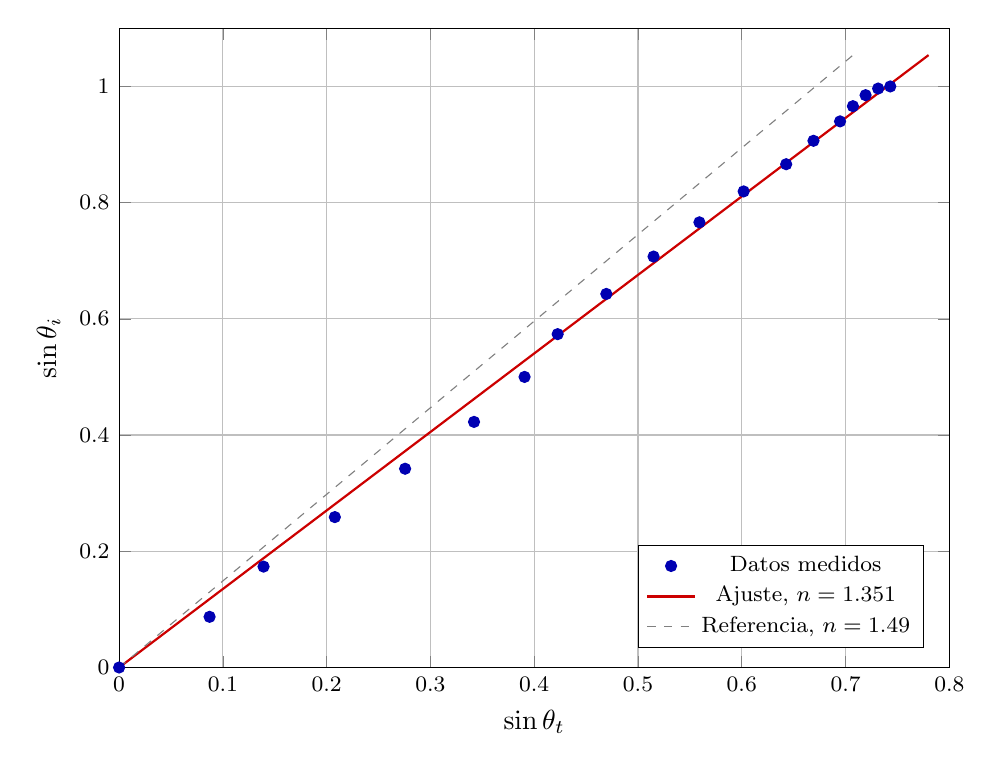
\begin{tikzpicture}
\begin{axis}[
    width=\columnwidth,
    height=0.8\columnwidth,
    xlabel={$\sin\theta_t$},
    ylabel={$\sin\theta_i$},
    xmin=0, xmax=0.8,
    ymin=0, ymax=1.1,
    grid=major,
    legend pos=south east,
    legend style={font=\footnotesize},
    tick label style={font=\footnotesize},
]
\addplot[only marks, mark=*, color=blue!70!black] coordinates {
    (0,0) (0.0872,0.0872) (0.1392,0.1736) (0.2079,0.2588) (0.2756,0.3420)
    (0.3420,0.4226) (0.3907,0.5000) (0.4226,0.5736) (0.4695,0.6428)
    (0.5150,0.7071) (0.5592,0.7660) (0.6018,0.8192) (0.6428,0.8660)
    (0.6691,0.9063) (0.6947,0.9397) (0.7071,0.9659) (0.7193,0.9848)
    (0.7314,0.9962) (0.7431,0.9998)
};
\addlegendentry{Datos medidos}
\addplot[domain=0:0.78, samples=2, thick, color=red!80!black] {1.351*x};
\addlegendentry{Ajuste, $n = 1.351$}
\addplot[domain=0:0.71, samples=2, dashed, color=gray] {1.49*x};
\addlegendentry{Referencia, $n = 1.49$}
\end{axis}
\end{tikzpicture}
\captionof{figure}{Seno del ángulo de incidencia contra seno del ángulo de refracción con la luz entrando por la cara plana.}
\label{fig:plana}
\end{center}

\subsection{Luz entrando por la cara curva}
Aquí la luz cruza la cara curva sin doblarse y se refracta al salir por la plana, es decir, va del acrílico al aire. La tabla \ref{tab:curva} reúne los datos hasta 40 grados. En este caso el índice de cada pareja se calcula como $n = \sin\theta_t / \sin\theta_i$.

\begin{center}
\begin{tabular}{ccccc}
\hline
$\theta_i$ & $\theta_t$ & $\sin\theta_i$ & $\sin\theta_t$ & $n$ \\
(grados) & (grados) & & & \\
\hline
0  & 0  & 0      & 0      & ---   \\
5  & 7  & 0.0872 & 0.1219 & 1.398 \\
10 & 15 & 0.1736 & 0.2588 & 1.490 \\
15 & 23 & 0.2588 & 0.3907 & 1.510 \\
20 & 30 & 0.3420 & 0.5000 & 1.462 \\
25 & 39 & 0.4226 & 0.6293 & 1.489 \\
30 & 48 & 0.5000 & 0.7431 & 1.486 \\
35 & 60 & 0.5736 & 0.8660 & 1.510 \\
40 & 74 & 0.6428 & 0.9613 & 1.495 \\
\hline
\end{tabular}
\captionof{table}{Ángulos de incidencia, dentro del acrílico, y de refracción, en el aire, con la luz entrando por la cara curva.}
\label{tab:curva}
\end{center}

Ahora el rayo se aleja de la normal, y cada vez más rápido. Entre 35 y 40 grados de incidencia el ángulo de salida brincó de 60 a 74 grados, y en esa zona empezó a verse además un rayo reflejado débil dentro de la lente. Con la ecuación \eqref{eq:recta2} se obtuvo la recta de la figura \ref{fig:curva}:
\begin{equation}
\sin\theta_t = 1.494 \, \sin\theta_i , \qquad R^2 = 0.9997 .
\label{eq:ajuste_curva}
\end{equation}

\begin{center}
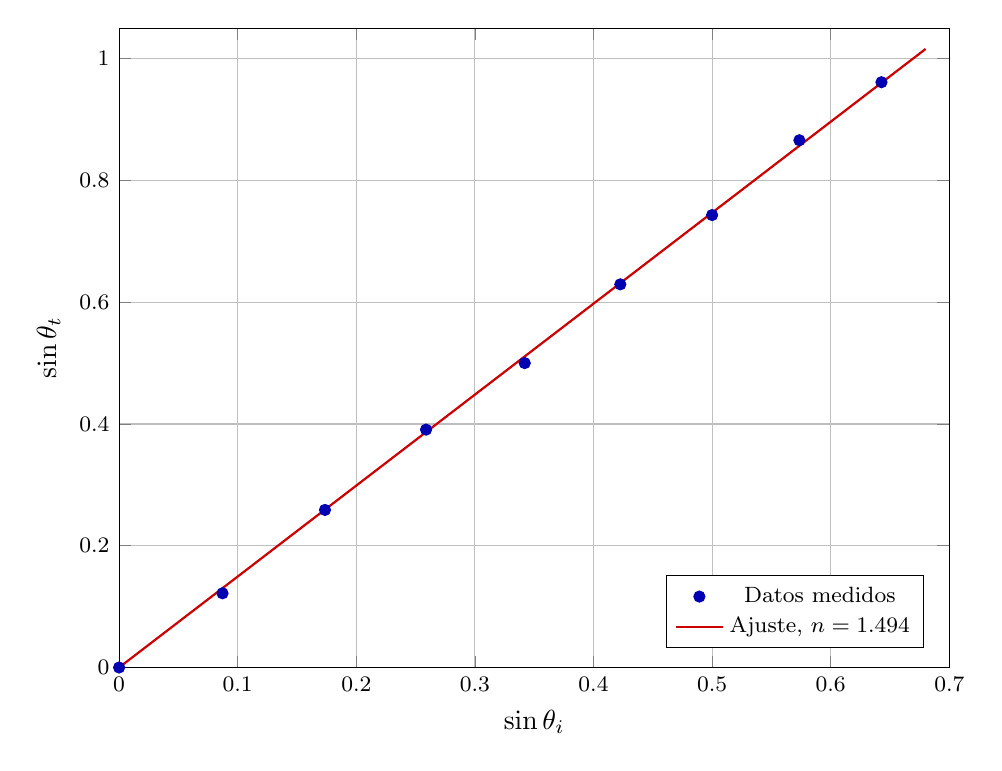
\begin{tikzpicture}
\begin{axis}[
    width=\columnwidth,
    height=0.8\columnwidth,
    xlabel={$\sin\theta_i$},
    ylabel={$\sin\theta_t$},
    xmin=0, xmax=0.7,
    ymin=0, ymax=1.05,
    grid=major,
    legend pos=south east,
    legend style={font=\footnotesize},
    tick label style={font=\footnotesize},
]
\addplot[only marks, mark=*, color=blue!70!black] coordinates {
    (0,0) (0.0872,0.1219) (0.1736,0.2588) (0.2588,0.3907) (0.3420,0.5000)
    (0.4226,0.6293) (0.5000,0.7431) (0.5736,0.8660) (0.6428,0.9613)
};
\addlegendentry{Datos medidos}
\addplot[domain=0:0.68, samples=2, thick, color=red!80!black] {1.494*x};
\addlegendentry{Ajuste, $n = 1.494$}
\end{axis}
\end{tikzpicture}
\captionof{figure}{Seno del ángulo de refracción contra seno del ángulo de incidencia con la luz entrando por la cara curva.}
\label{fig:curva}
\end{center}

\subsection{Reflexión total interna}
De 45 grados en adelante ya no salió ningún rayo por la cara plana. Toda la luz se reflejó hacia dentro de la lente, y en la escala de la mesa ese rayo reflejado se leyó del otro lado del círculo, de modo que su ángulo respecto a la normal es $180$ menos la lectura. La tabla \ref{tab:reflexion} lo muestra.

\begin{center}
\begin{tabular}{ccc}
\hline
$\theta_i$ & Lectura & $\theta_r = 180 - \text{lectura}$ \\
(grados) & (grados) & (grados) \\
\hline
45 & 135 & 45 \\
50 & 130 & 50 \\
55 & 126 & 54 \\
60 & 121 & 59 \\
65 & 116 & 64 \\
70 & 111 & 69 \\
75 & 106 & 74 \\
80 & 102 & 78 \\
85 & 96  & 84 \\
90 & 90  & 90 \\
\hline
\end{tabular}
\captionof{table}{Ángulo del rayo reflejado cuando ya no hay rayo transmitido.}
\label{tab:reflexion}
\end{center}

El ángulo reflejado coincide con el de incidencia con una diferencia de dos grados como máximo, que es lo que pide la ley de la reflexión.
